\documentclass[12pt, a4paper, usenames, dvipsnames]{article}

\usepackage[margin=1in]{geometry}
%\usepackage[colorlinks=true,linkcolor=black,citecolor=black]{hyperref}
\usepackage[small]{titlesec}

\usepackage[longnamesfirst]{natbib}
  \bibliographystyle{sp}
  \bibpunct[:]{(}{)}{,}{a}{}{,}
  \setlength{\bibsep}{0ex}
  \newcommand{\cites}[1]{\citeauthor*{#1}'s (\citeyear{#1})}
  \newcommand{\citeals}[1]{\citeauthor*{#1}'s \citeyear{#1}}

\usepackage{amssymb,amsmath,amsmath}


\usepackage{linguex}
  \renewcommand{\firstrefdash}{}

%\setlength{\parskip}{3pt}
\setlength{\parindent}{0pt}

\usepackage{tikz,tikz-qtree}
\usetikzlibrary{arrows,positioning,fit}
\usepackage[normalem]{ulem}
%\usepackage{mdframed}

\usepackage{braket, url}
\usepackage{colortbl, multirow, makecell, tabularx, caption, subcaption,  wrapfig, booktabs, wrapfig}

\usepackage{theorem}
  \theorembodyfont{\upshape}
  \newtheorem{dfn}{Definition}
  \newtheorem{thm}{Theorem}
  \newtheorem{lmm}{Lemma}
  \newtheorem{syn}{Syntax}

\def\co{\colon\thinspace}

%\usepackage{mathabx}
\usepackage{stix}
%\newcommand{\sem}[2][]{\mbox{\ensuremath{\left\lsemantic\textsf{#2}\right\rsemantic^{#1}}}}
\newcommand{\sem}[2][]{\mbox{\ensuremath{\left\lBrack\text{#2}\right\rBrack^{#1}}}}


\title{}
\author{
	Yasutada Sudo\\UCL\\
	\texttt{y.sudo@ucl.ac.uk}
	}
\date{\today}

\DeclareRobustCommand{\van}[3]{#2}

\makeatletter
\renewcommand{\printExNo}{%
  \@ifnextchar[{\complexExNo}{%
    \hyperlink{ExNo.\thetmpaEx}{%
      \if@noftnote\theExLBr\else\theFnExLBr\fi
      \thetmpaEx
      \if@noftnote\theExRBr\else\theFnExRBr\fi
    }%
    \xspace
  }%
}
\makeatother


\begin{document}

\begin{itemize}
  \item Two utterances: `some' and `all'
  \item Two possible states/meanings: \texttt{sbna} and \texttt{all}.
\end{itemize}


\section{Standard RSA}
\begin{align*}
  L_0(w|u) & \propto \sem[w]{\(u\)}P(w) & \text{Literal listener \(L_0\)}
  \\
  S_n(u|w) & \propto \exp(\lambda\log L_{n-1}(w|u)) - c(u) & \text{Pragmatic speaker}\\
  L_n(w|u) & \propto S_n(u|w) P(w) & \text{Pragmatic listener}
\end{align*}

We assume a completely rational speaker \(\lambda =1\). Since two utterances `some' and `all' are not so different in cost, we ignore the cost term.


\subsection{Uniform prior} 
With a uniform prior, \(P(\texttt{all})=P(\texttt{sbna})=0.5\), we get the correct result.

\begin{align*}
  L_0(\texttt{all}|\text{`all'}) & = 1\\
%  L_0(\texttt{sbna}|\text{`all'}) & = 0\\
%  \\
  L_0(\texttt{all}|\text{`some'}) & = \frac{P(\texttt{all})}{P(\texttt{all})+P(\texttt{sbna})} = 0.50\\
  %L_0(\texttt{sbna}|\text{`some'}) & = \frac{P(\texttt{sbna})}{P(\texttt{all})+P(\texttt{sbna})} = 0.5\\
   S_1(\text{`some'}|\texttt{all}) & = 0.33\\
   L_1(\texttt{all}|\text{`some'}) & = 0.25\\
   S_2(\text{`some'}|\texttt{all}) & = 0.2\\
\end{align*}



\subsection{The problem of skewed priors}
However, when the prior is skewed, we get the wrong results (Spector, Fox \& Katzir, Degen et al.). For example, with \(P(\texttt{all})=0.9$, $P(\texttt{sbna})=0.1\):
\begin{align*}
  L_0(\texttt{all}|\text{`all'}) & = 1\\
  L_0(\texttt{all}|\text{`some'}) & = 0.9\\
  S_1(\text{`some'}|\texttt{all}) & = 0.47\\
  L_1(\texttt{all}|\text{`some'}) & = 0.81\\
  S_2(\text{`some'}|\texttt{all}) & = 0.44\\
  L_2(\texttt{all}|\text{`some'}) & = 0.80\\
\end{align*}
The values decrease here, but will not improve much. See Figure \ref{fig:rsa}.

\begin{figure}[!htb]
  \begin{subfigure}{.48\linewidth} 
    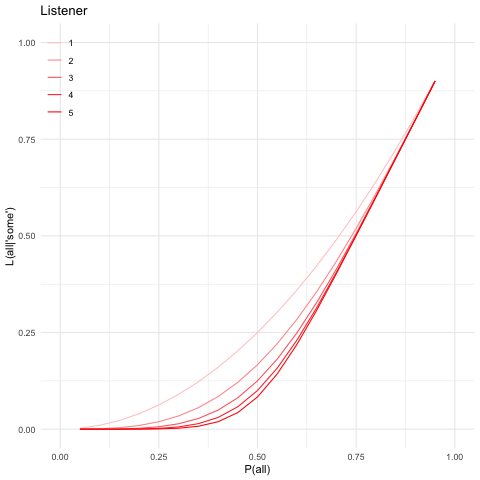
\includegraphics[width=\textwidth]{graphs/RSA-L.png}
    \caption{\(L_n(\texttt{all}|\text{`some'})\) for \(1\leq n\leq 5\)}
  \end{subfigure}
  \begin{subfigure}{.48\linewidth} 
    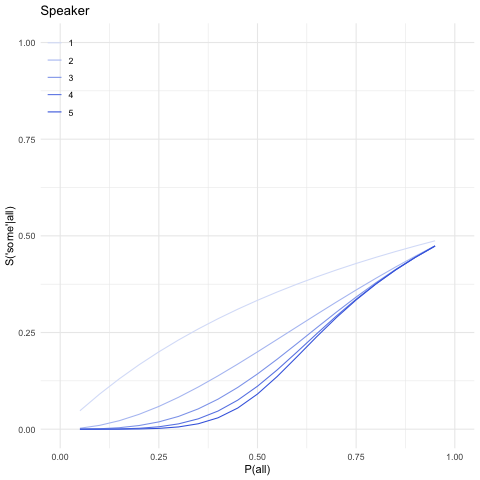
\includegraphics[width=\textwidth]{graphs/RSA-S.png}
    \caption{\(S_n(\text{`some'}|\texttt{all})\) for \(1\leq n\leq 5\)}
  \end{subfigure}
  \caption{Probabilities of `some' meaning \texttt{all} as a function of \(P(\texttt{all})\) in RSA.}
  \label{fig:rsa}
\end{figure}

When \(P(\texttt{all})\) is high, the speaker is about 50\% likely to use `some' to mean \texttt{all} (because they almost randomly choose between `all' and `some'), and the listener is very likely to interpret `some' as \texttt{all} (because it's more likely to be true).


\section{Stalnakerian Listener}

\begin{wrapfigure}{r}{.4\textwidth}
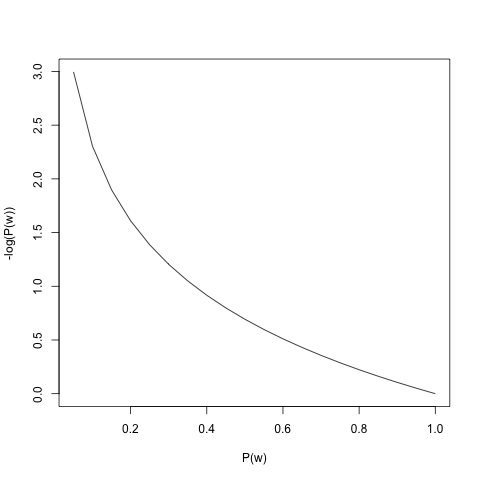
\includegraphics[width=.4\textwidth]{graphs/info.png}
\end{wrapfigure}
The intuition is that when \(P(\texttt{all})\) is high, it does not need to be linguistically conveyed that \texttt{all} is the case, because the utterance would be underinformative. Knowing that the speaker would avoid redundancy, the rational listener should prefer the most informative interpretation of the utterance.



In order to implement this, let's make use of the \emph{surprisal} (information content) of learning that $w$ is the case, \(-\log P(w)\).\footnote{Using the same Literal Listener as the standard RSA only changes the initial level.}

\begin{align*}
%  L_0(w|u) & \propto \textsf{info}(u|w,\textsf{Lex})P(w) & \text{Literal listener \(L_0\)}
  L_0(w|u) & \propto -\log P(w) \times \sem[w]{$u$}P(w) & \text{Literal listener}\\
  L_n(w|u) & \propto -\log P(w) \times S_n(u|w)P(w) & \text{Pragmatic listener}\\
  S_n(u|w) & \propto \exp(\lambda\log L_{n-1}(w|u)) & \text{Pragmatic speaker}
\end{align*}
With a uniform prior, \(P(\texttt{all})=P(\texttt{sbna})=0.5\), the results are not so different from the standard RSA.
\begin{align*}
%  L_0(\texttt{all}|\text{`all'}) & = 1\\
%  \\
  L_0(\texttt{all}|\text{`some'}) & = 0.50\\
  S_1(\text{`some'}|\texttt{all}) & = 0.33\\
  L_1(\texttt{all}|\text{`some'}) & = 0.25\\
  S_2(\text{`some'}|\texttt{all}) & = 0.20\\  
  L_2(\texttt{all}|\text{`some'}) & = 0.17\\
\end{align*}

The results are better with the skewed prior, \(P(\texttt{all})=0.9, P(\texttt(sbna))=0.1\):
\begin{align*}
%  L_0(\texttt{all}|\text{`all'}) & = 1\\
%  \\
  L_0(\texttt{all}|\text{`some'}) & = 0.29\\
  S_1(\text{`some'}|\texttt{all}) & = 0.23\\
  L_1(\texttt{all}|\text{`some'}) & = 0.09\\
  S_2(\text{`some'}|\texttt{all}) & = 0.08\\  
  L_2(\texttt{all}|\text{`some'}) & = 0.03\\
\end{align*}

However, we now have a problem with a different skewed prior, \(P(\texttt{all})=0.1, P(\texttt(sbna))=0.9\):
\begin{align*}
%  L_0(\texttt{all}|\text{`all'}) & = 1\\
%  \\
  L_0(\texttt{all}|\text{`some'}) & = 0.71\\
  S_1(\text{`some'}|\texttt{all}) & = 0.41\\
  L_1(\texttt{all}|\text{`some'}) & = 0.50\\
  S_2(\text{`some'}|\texttt{all}) & = 0.33\\ 
  L_2(\texttt{all}|\text{`some'}) & = 0.45\\
\end{align*}
\begin{figure}[!htb]
  \begin{subfigure}{.48\linewidth} 
    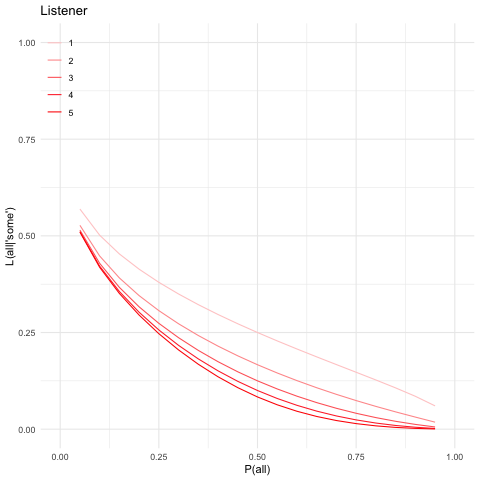
\includegraphics[width=\textwidth]{graphs/sRSA-L.png}
    \caption{\(L_n(\texttt{all}|\text{`some'})\) for \(1\leq n\leq 5\)}
  \end{subfigure}
  \begin{subfigure}{.48\linewidth} 
    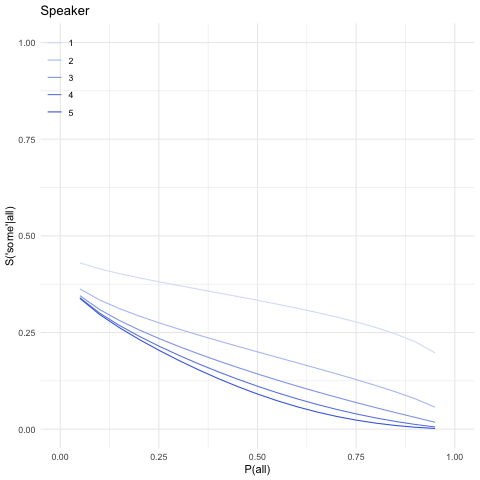
\includegraphics[width=\textwidth]{graphs/sRSA-S.png}
    \caption{\(S_n(\text{`some'}|\texttt{all})\) for \(1\leq n\leq 5\)}
  \end{subfigure}
  \caption{Probabilities of `some' meaning \texttt{all} as a function of \(P(\texttt{all})\) in RSA with the Stalnakerian Listener.}
  \label{fig:rsa}
\end{figure}


In this model, when \(P(\texttt{all})\) is low, it makes sense to mean \texttt{all} with `some', because \texttt{all} is highly informative while \texttt{sbna} is not. Knowing this, the speaker can choose `some' to express \texttt{all}.


\section{Maxent Speaker}

When \(P(\texttt{all})\) is low, the speaker shouldn't use `some' to express \texttt{all}, because it could potentially receive an underinformative reading, while `all' is a solid means of expressing it because it always means \texttt{all}.

The speaker model of the standard RSA doesn't capture this, because the speaker just chooses the most reliable message to convey $w$ with respect to the listener model $L$, by maximizing the negative surprisal $\log L(w|u)$. So the speaker doesn't directly consider what the alternative meaning would do.

With the Stalnakerian Listener, this is indirectly captured. They try to avoid underinformative meaning, so when the Speaker maximizes the negative surprisal $\log L(w|u)$, the relatively more informative meaning will become more likely.

But I think it makes sense to directly encode this consideration in the speaker model. The idea is that the speaker tries to maximize the average surprisal, or \emph{entropy}, $H(u|L)$, of message $u$ relative to the listener model $L$.
\[
S_n(u|w) \propto \exp(\lambda (\underbrace{\log L_{n-1}(w|u)}_{\text{\normalsize reliability}} + \underbrace{H(u|L_{n-1})}_{\text{\normalsize entropy wrt $L_{n-1}$}}))
\]
The entropy of message $u$ with respect to the listener model $L$ is defined as the following cross entropy:
\[
H(u|L) = \sum_{w'} \overbrace{-\log P(w')}^{\text{\normalsize impact on CG}}\times \underbrace{L(w'|u)}_{\text{\normalsize Probability of $u$ meaning $w'$ wrt to $L$}}
\]


This model, however, doesn't completely solve the problem. See Figure \ref{fig:shannon} (It's computationally heavy, so I could only compute up to Level 4).

\begin{figure}[!htb]
  \begin{subfigure}{.48\linewidth} 
    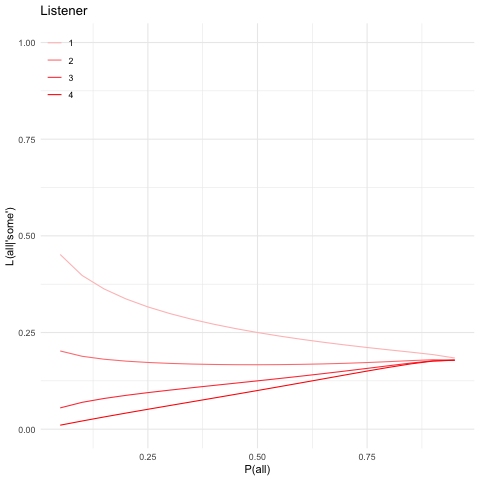
\includegraphics[width=\textwidth]{graphs/shannonRSA-L.png}
    \caption{\(L_n(\texttt{all}|\text{`some'})\) for \(1\leq n\leq 4\)}
  \end{subfigure}
  \begin{subfigure}{.48\linewidth} 
    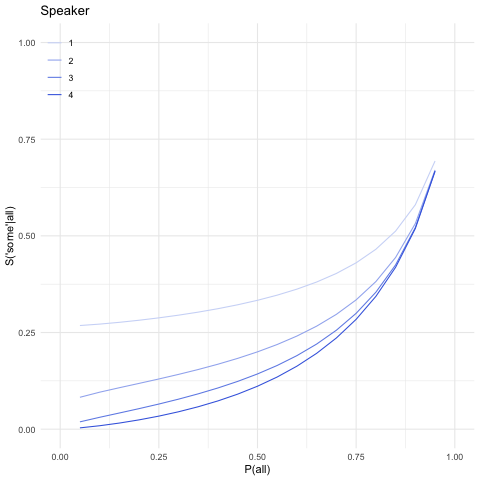
\includegraphics[width=\textwidth]{graphs/shannonRSA-S.png}
    \caption{\(S_n(\text{`some'}|\texttt{all})\) for \(1\leq n\leq 4\)}
  \end{subfigure}
  \caption{Probabilities of `some' meaning \texttt{all} as a function of \(P(\texttt{all})\) in RSA with the Stalnakerian Listener and Maxent Speaker.}
  \label{fig:shannon}
\end{figure}

In particular, it recreates the initial problem for the speaker. The reason is because the utility of meaning \texttt{all} is so high that this consideration overrides the reliability of the listener understanding `some' as \texttt{all}. To make the impact of the entropy smaller, let's regulate it via a constant $k$.
\[
S_n(u|w) \propto \exp(\lambda (\underbrace{\log L_{n-1}(w|u)}_{\text{\normalsize reliability}} + k\cdot\underbrace{H(u|L_{n-1})}_{\text{\normalsize entropy wrt $L_{n-1}$}}))
\]

With $k=0.5$, we obtain better results:
\begin{figure}[!htb]
  \begin{subfigure}{.48\linewidth} 
    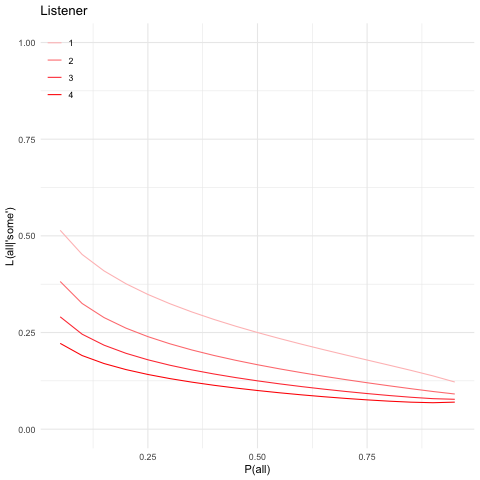
\includegraphics[width=\textwidth]{graphs/shannonRSA-L05.png}
    \caption{\(L_n(\texttt{all}|\text{`some'})\) for \(1\leq n\leq 4\)}
  \end{subfigure}
  \begin{subfigure}{.48\linewidth} 
    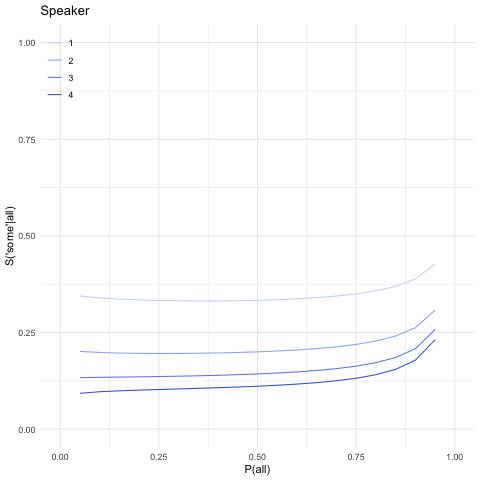
\includegraphics[width=\textwidth]{graphs/shannonRSA-S05.png}
    \caption{\(S_n(\text{`some'}|\texttt{all})\) for \(1\leq n\leq 4\)}
  \end{subfigure}
  \caption{Probabilities of `some' meaning \texttt{all} as a function of \(P(\texttt{all})\) in RSA with the Stalnakerian Listener and Maxent Speaker with $k=0.5$.}
  \label{fig:shannon05}
\end{figure}
But the numbers are still not very satisfactory.

In addition, a lower or higher value of $k$ will result in worse predictions (see the next page).
\begin{figure}[!htb]
  \begin{subfigure}{.48\linewidth} 
    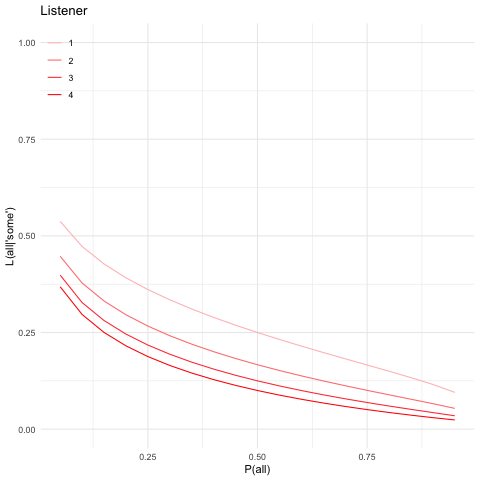
\includegraphics[width=\textwidth]{graphs/shannonRSA-L03.png}
    \caption{\(L_n(\texttt{all}|\text{`some'})\) for \(1\leq n\leq 4\), $k=0.3$}
  \end{subfigure}
  \begin{subfigure}{.48\linewidth} 
    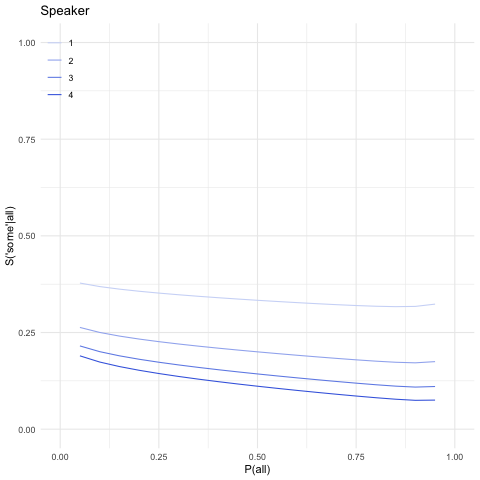
\includegraphics[width=\textwidth]{graphs/shannonRSA-S03.png}
    \caption{\(S_n(\text{`some'}|\texttt{all})\) for \(1\leq n\leq 4\), $k=0.3$}
  \end{subfigure}
  \begin{subfigure}{.48\linewidth} 
    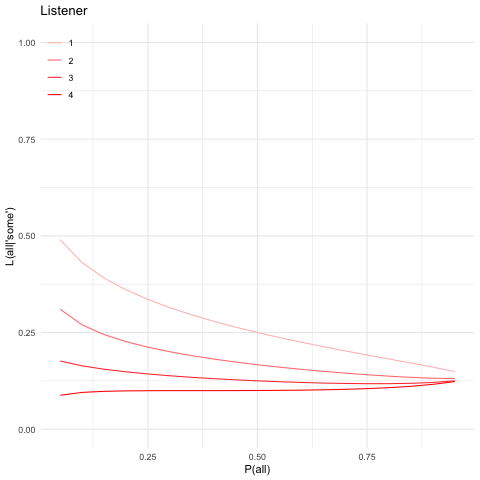
\includegraphics[width=\textwidth]{graphs/shannonRSA-L07.png}
    \caption{\(L_n(\texttt{all}|\text{`some'})\) for \(1\leq n\leq 4\), $k=0.7$}
  \end{subfigure}
  \begin{subfigure}{.48\linewidth} 
    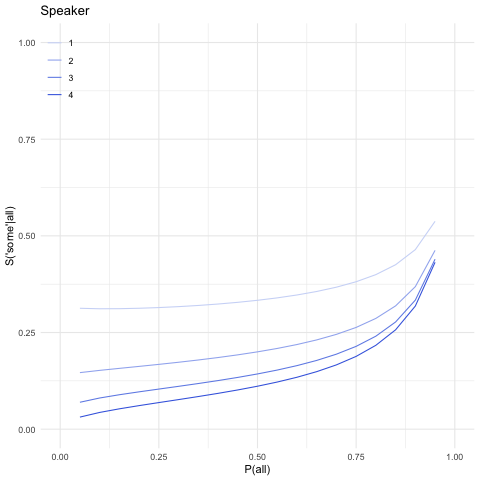
\includegraphics[width=\textwidth]{graphs/shannonRSA-S07.png}
    \caption{\(S_n(\text{`some'}|\texttt{all})\) for \(1\leq n\leq 4\), $k=0.7$}
  \end{subfigure}
\end{figure}


\bibliography{ling}
\end{document}
